\subsection{Server Subsystem}
The server layer subsystem will calculate the difference between the mean representative audio stored on the server and the input audio.
It runs continously and accepts POST requests containing audio and a target word.

\begin{figure}[h!]
	\centering
 	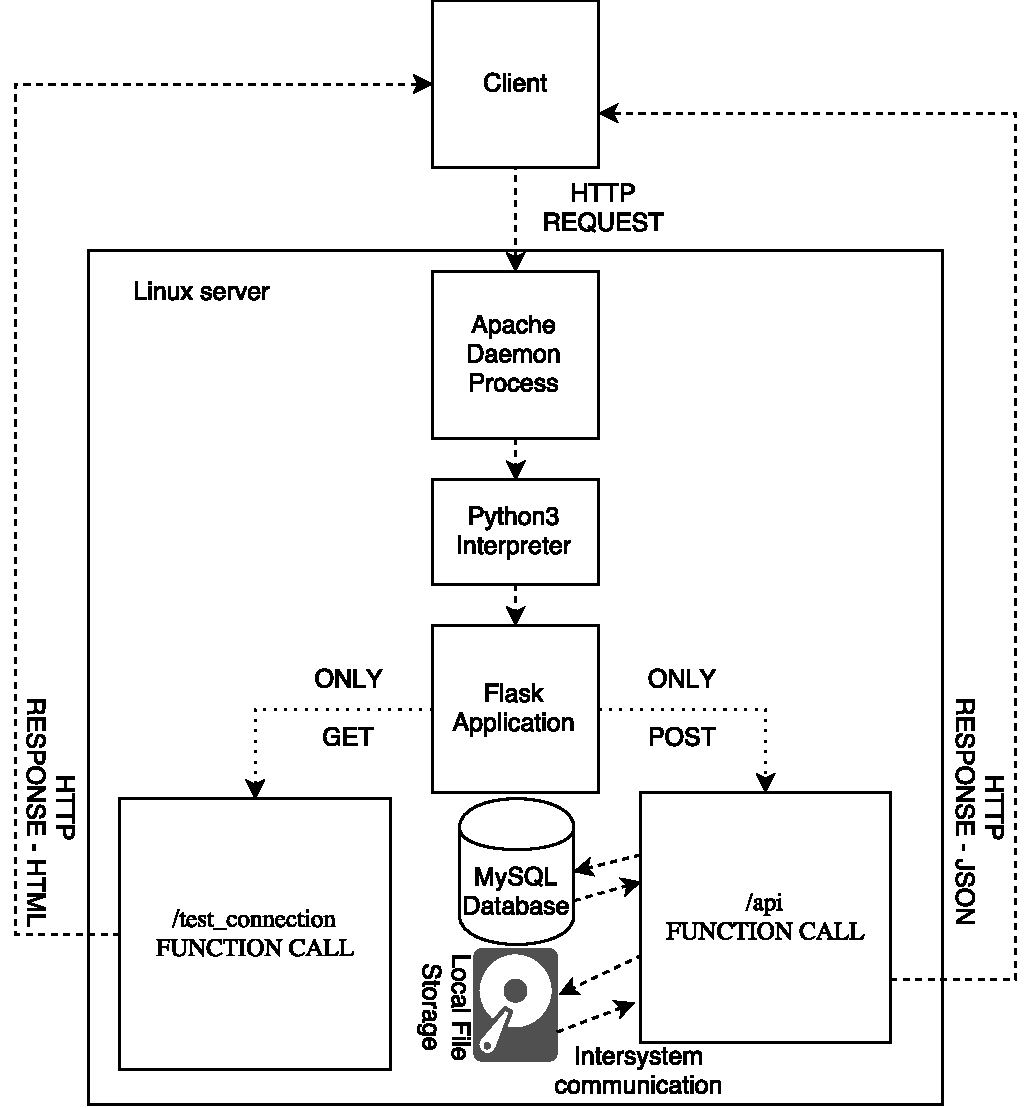
\includegraphics[width=\textwidth]{images/server_subsystems.pdf}
 \caption{Server subsystem diagram}
\end{figure}

\subsubsection{Assumptions}
    The client will only send queries which the server can answer. At the heart of this assumption is the idea that POST requests should be sent in a specific format.

\subsubsection{Responsibilities}
    The server layer subsystem will be responsible for:
    \begin{itemize}
        \item Accepting and maintaining a POST request.
        \item Temporarily storing and removing when done the input audio file.
        \item Extracting features from each locally stored audio sample and aggregate into a single representative feature set.
        \item Extracting the feature set from the input audio sample and aggregate into a single representative feature set.
        \item Concatenate, normalize, and compare each representative feature set.
        \item Return a score for the difference.
    \end{itemize}

\subsubsection{Subsystem Interfaces}
    \begin {table}[H]
        \begin{center}
            \begin{tabular}{ | p{1cm} | p{6cm} | p{4cm} | p{5cm} |}
                \hline
                ID & Description & Inputs & Outputs \\ \hline
                \#1 & \texttt{/test\_connection/} & \pbox{4cm}{} & \pbox{5cm}{\texttt{HTML=HELLO WORLD}}  \\ \hline
                \#2 & \texttt{/api/} & \pbox{4cm}{\texttt{(word,word.mp3)}} & \pbox{5cm}{\vspace{0.5em}\texttt{JSON=\{word:word, score:difference\_measure\}}\vspace{0.5em}}  \\ \hline
            \end{tabular}
            \label{server_sys}
            \caption{Server Subsystem interfaces} 
        \end{center}
    \end{table}
